\documentclass[unknownkeysallowed]{beamer}

\mode<presentation> {
\usetheme{Copenhagen}
\usecolortheme{beaver}
}

\usepackage{graphicx} % Allows including images

\usepackage[utf8]{inputenc}
\usepackage[slovene]{babel}
\usepackage{algorithmicx, algpseudocode}

\usepackage{varwidth}

\usepackage[labelformat=empty]{caption}

\title[Network analysis of metabolic subsystems]{Network analysis of metabolic subsystems}

\author{Rok Novosel and Matija Čufar} % Your name
\institute[]
{
Faculty of Computer and Information Science \\
\medskip
}
\date{\today}

\begin{document}

\begin{frame}
\titlepage % Print the title page as the first slide
\end{frame}

\begin{frame}{Network analysis of metabolic subsystems}
  \includegraphics[width=.5\textwidth]{ch}
  \includegraphics[width=.5\textwidth]{network}
\end{frame}

\begin{frame}{Network stats}
  \centering
  \includegraphics[height=.6\textheight]{../../plots/degreesmall2}

  \begin{tabular}{l|l|l|l|l|l}
    $|V|$ & $|E|$ & $\langle C \rangle$ & $E_{90}$ & $\rho$ & $\langle k \rangle$ \\ \hline
    6,663 & 656,609 & 0.012 & 15 & 0.015 & 194.1
  \end{tabular}
\end{frame}

\begin{frame}{Community detection}

  \centering
  \begin{tabular}{l|l}
    Algorithm & NMI \\ \hline
    Louvain Modularity & 0.10 \\
    Clauset-Newman-Moore & 0.27 \\
    Infomap & N/A \\
    Girvan-Newman & N/A
  \end{tabular}

\end{frame}

\begin{frame}{Motif based community detection}
  \includegraphics[width=\textwidth]{benson}
  \footnote{source: http://snap.stanford.edu/higher-order/}
\end{frame}

\begin{frame}{Motif based community detection and motif significances}
  \centering
  \begin{tabular}{l|lllllll}
    &
    \includegraphics[height=0.10\textheight]{M1-plain} &
    \includegraphics[height=0.10\textheight]{M2-plain} &
    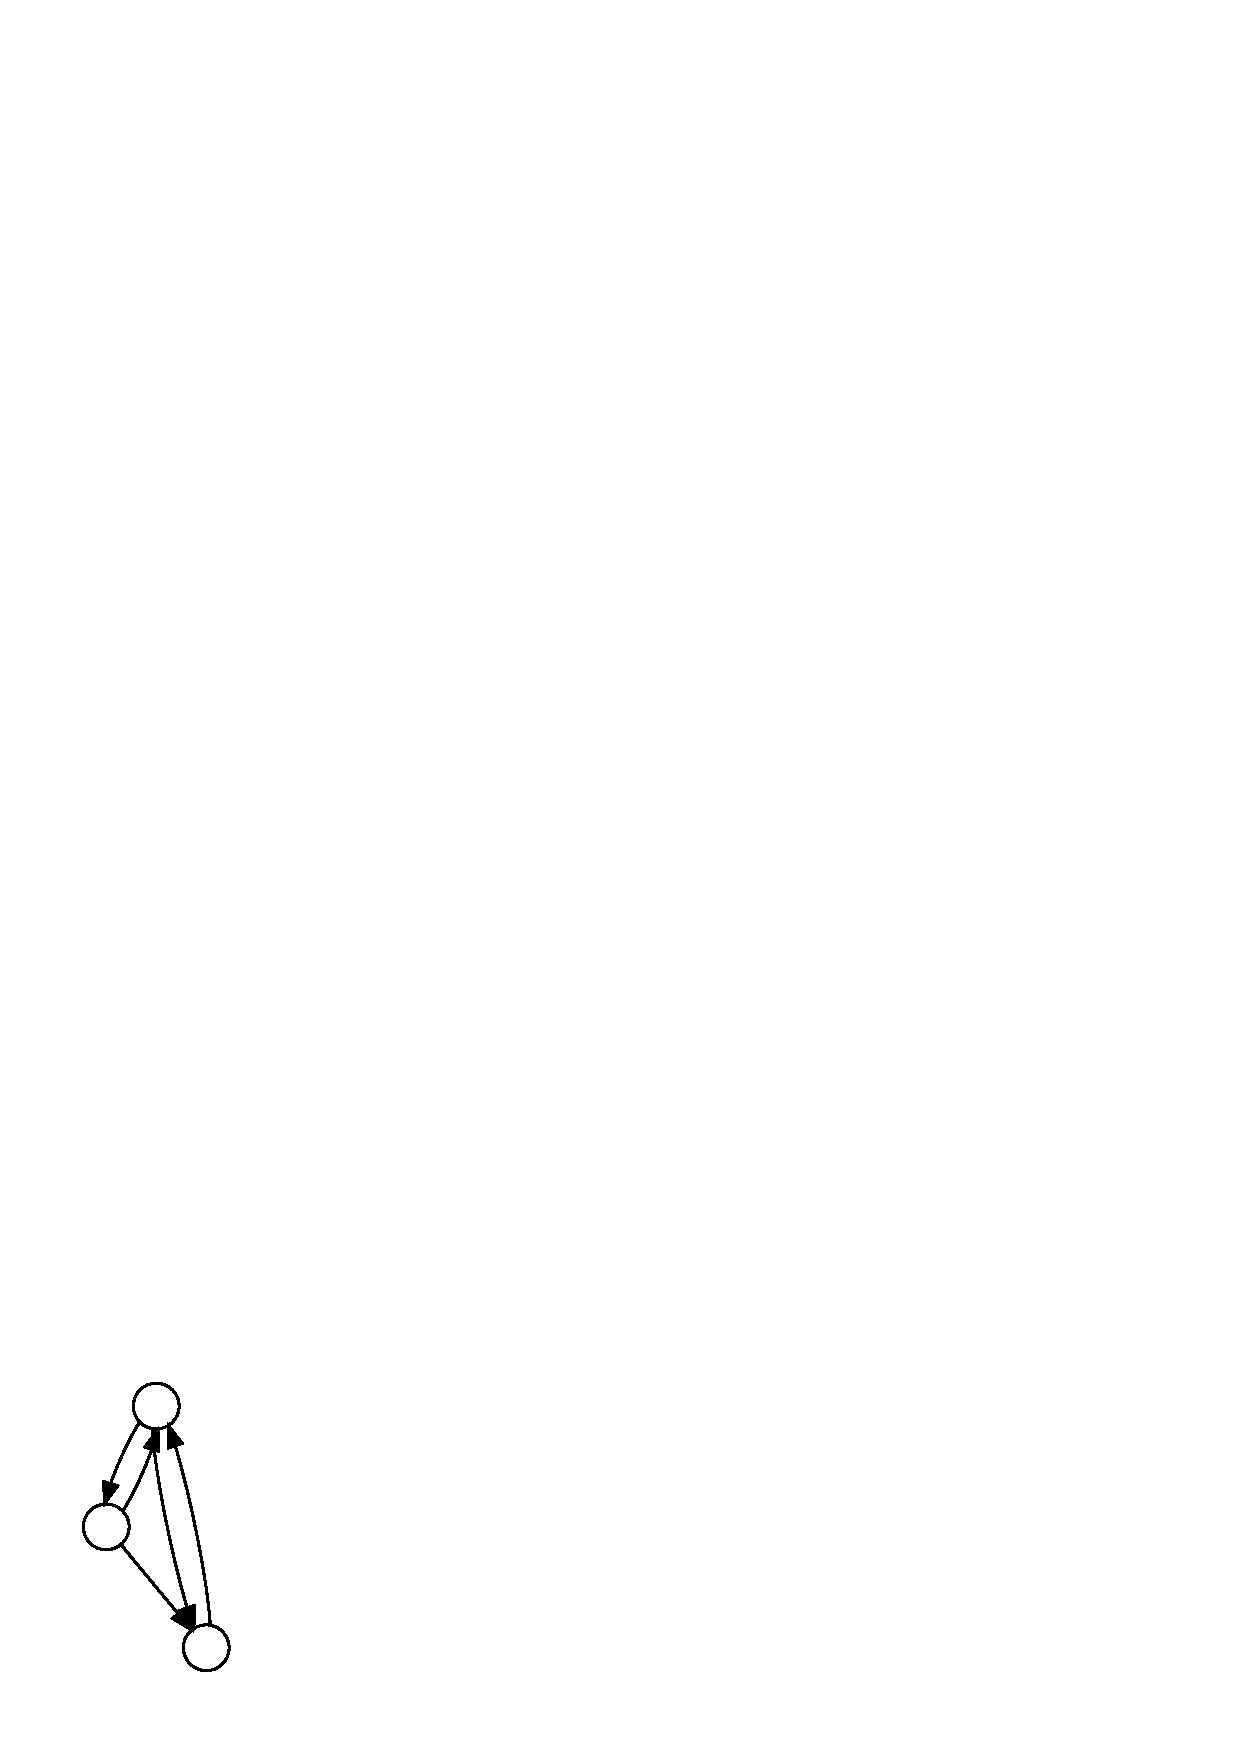
\includegraphics[height=0.10\textheight]{M3-plain} &
    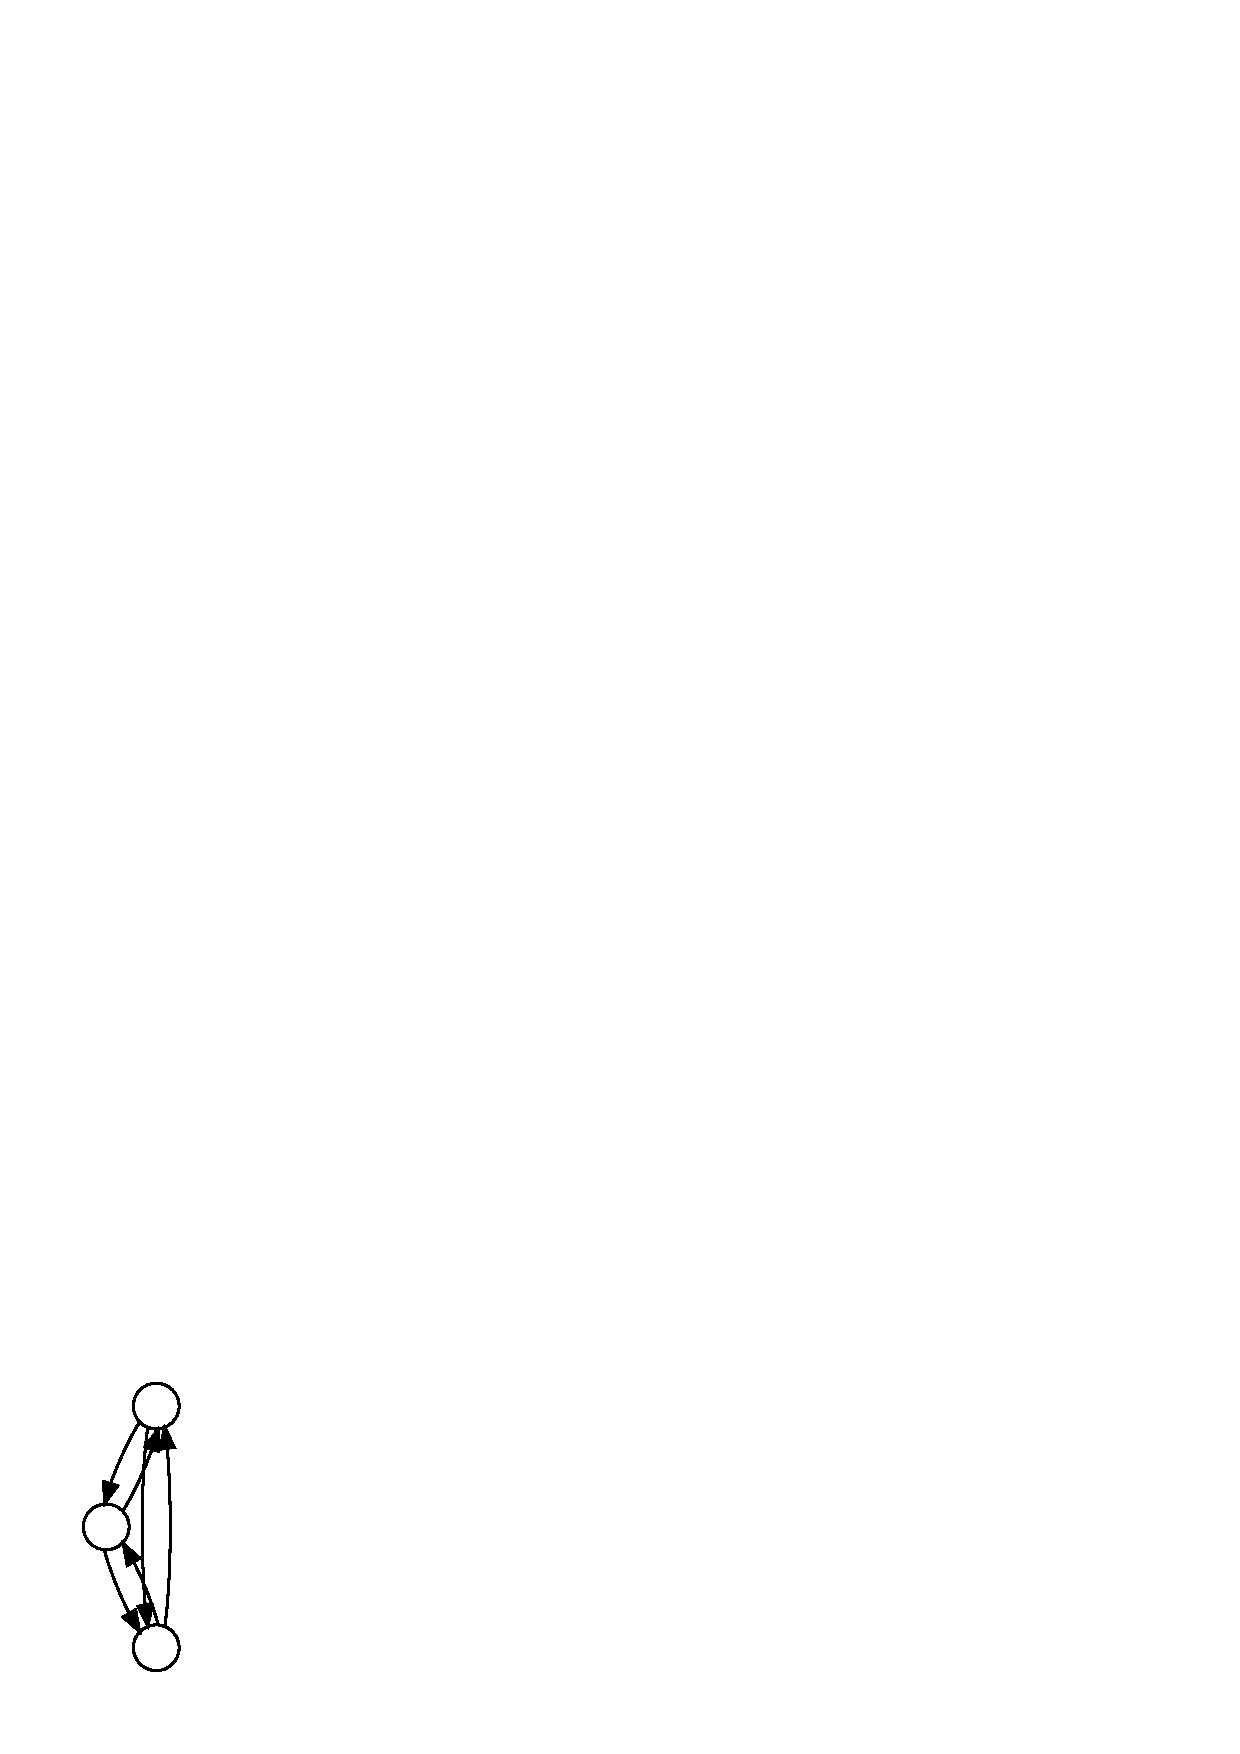
\includegraphics[height=0.10\textheight]{M4-plain} &
    \includegraphics[height=0.10\textheight]{M5-plain} &
    \includegraphics[height=0.10\textheight]{M6-plain} &
    \includegraphics[height=0.10\textheight]{M7-plain} \\ \hline
    motif & M1 & M2 & M3 & M4 & M5 & M6 & M7
    \\ \hline
    $Z$ & -379.0 & 496.4 & 6,523 & 1,171,385 & 1,055 & 3,566 & 4,604 \\
    NMI & 0.44 & 0.40 & 0.48 & 0.64 & 0.23 & 0.43 & 0.46 \\ \hline \hline
    \noalign{\smallskip}
    &
    \includegraphics[height=0.10\textheight]{M8-plain} &
    \includegraphics[height=0.10\textheight]{M9-plain} &
    \includegraphics[height=0.10\textheight]{M10-plain} &
    \includegraphics[height=0.10\textheight]{M11-plain} &
    \includegraphics[height=0.10\textheight]{M12-plain} &
    \includegraphics[height=0.10\textheight]{M13-plain} & \\ \hline
    motif & M8 & M9 & M10 & M11 & M12 & M13 & \\ \hline
    $Z$ & 1,411 & -867.2 & 2,599 & 1,293 & 1,387 & 40,286 & \\
    NMI & 0.11 & 0.09 & 0.09 & 0.20 & 0.23 & 0.42 & \\
  \end{tabular}

  \begin{equation*}
    Z = \frac{n - \mu_{\mathrm{rand}}}{\sigma_{\mathrm{rand}}}
  \end{equation*}
\end{frame}

\end{document}
